\section{TUPLES}
Sebuah tupel adalah urutan objek Python yang tidak berubah. Tupel adalah urutan, seperti daftar. Perbedaan antara tupel dan daftar adalah, tupel tidak dapat diubah tidak seperti daftar dan tupel menggunakan tanda kurung, sedangkan daftar menggunakan tanda kurung siku. 
Tuple juga merupakan tipe data yang berurut (sequence data type) yang fungsinya hampir sama List. Namun Tuple juga berbeda sifatnya, yaitu Tuple bersifat immutable maksudnya data di dalam Tuple tidak dapat diubah atau dihapuskan. Sebuah Tuple terdiri dari beberapa nilai yang dipisah oleh tanda koma \(‘,’\). Tidak seperti List, tipe data Tuple ditandai dengan tanda kurung \"()\".
Ini adalah contohnya, 

\section{Perbedaan antara list dengan tuple} 
\begin{enumerate}
\item Nilai dalam Tuple tidak bisa diganti. 
\item Kalau dalam List diawali dan diakhiri dengan tanda kurung siku [], Tuple dimulai dan ditutup dengan tanda kurung \(\). 
\end{enumerate}

Nilai-nilai pada Tuple yang sudah tentukan pada awal program tidak akan bisa diganti sampai akhir programnya. Dan tentunya index pada tuple selalu dimulai dari angka 0 

Membuat Tuple sangatlah mudah, nilai-nilai dapat dipisahkan dengan tanda koma. Seperti contoh di bawah ini : 
\begin{verbatim}
Tup1 = ("awal","tengah","akhir", 1,2); 

months = ('January','February','March','April','May','June','July','August','September','October','November',' December'); 
 \end{verbatim}
Berikut ini contoh membuat Tuple, kemudian menampilkan nilai, update \(dalam hal ini bukan meng-update nilai dalam Tuple melainkan membuat Tuple baru dan kemudian digabungkan dengan yang lama\) dan delete Tuple \(menghapus Tuple, bukan menghapus nilai dalam Tuple\). 
\begin{verbatim}
>>> NamaSiswa = ("Indra Riksa", "Agien Farhan", "Saryoni", "Berlin", "Kindi") 
>>> NamaSiswa 
('Indra Riksa', 'Agien Farhan', 'Saryoni, 'Berlin', 'Kindi') 
\end{verbatim}
Kita dapat mengisi sebuah Tuple tanpa memakai tanda kurung, tapi hal ini tidak dianjurkan jika Tuple tersebut berisi data yang besar. Contoh di bawah ini jika kita ingin membuat Tuple bersarang, ada Tuple di dalam Tuple. 
\begin{verbatim}
>>> NamaKota = "Surabaya", "Jakarta" 
>>> NamaKota 
('Surabaya', 'Jakarta') 
>>> KotaBesar = NamaKota, ("Bandung", "Yogyakarta", "Medan") 
>>> KotaBesar 
(('Surabaya', 'Jakarta'), ('Bandung', 'Yogyakarta', 'Medan'))
\end{verbatim}
Sesuai dengan yang sudah dibahas di awal tadi, perbedaan utama dari Tuple dan List yaitu : 
Tuple bersifat immutable \(tetap\), kita tidak diizinkan untuk mengganti nilai yang ada atau menghapus data yang ada dalam Tuple tersebut. Jika kita menghapus atau mengubah data yang sudah ada sebelumnya, maka pesan kesalahan akan di tampilkan oleh interpreter Python. 
\begin{verbatim}
>>> NamaKota[1] = \"Medan\" 
Traceback (most recent call last): 
File "", line 1, in 
NamaKota[1] = \"Medan\" 

TypeError: 'tuple' object does not support item assignment 
\end{verbatim}
Kita dapat menggunakan indeks atau irisan untuk mengakses nilai yang ada di dalam Tuple. Berikut contohnya, 
\begin{verbatim}
>>> NamaSiswa[1] 
'Indra Riksa' 
>>> NamaSiswa[0:2] 
('Indra Riksa', 'Agien Farhan') 
>>> KotaBesar[:2] 
(('Surabaya', 'Jakarta'), ('Bandung', 'Yogyakarta', 'Medan')) 
>>> KotaBesar[1][0] 
'Bandung' 

>>> TupleAku = ("a", 2, 3, 4) 
>>> TupleAku 
('a', 2, 3, 4) 
>>> TupleDia = ("b", 5, 6, 7) 
>>> TupleDia 
('b', 5, 6, 7) 
>>> TupleGab = TupleAku + TupleDia 
>>> TupleGab 
('a', 2, 3, 4, 'b', 5, 6, 7) 
\end{verbatim}
Contoh di atas, dua Tuple dibuat secara terpisah, TupleAku dan TupleDia. 
Dua Tuple ini dicocokkan pada Tuple lainnya TupleGab menggunakan operator +.
Perlu dicatat bahwa TupleGab berisi nilai dari TupleAku dan TupleDia. 
Metode ini dapat digunakan untuk menambahkan elemen data lain pada sebuah Tuple. 
\begin{verbatim}
>>> IniTuple = ("x", "y", "z") 
>>> IniTuple = IniTuple + ("a", "b")
>>> IniTuple 
('x', 'y', 'z', 'a', 'b') 
\end{verbatim}
Dan kita juga dapat membuat Tuple dengan objek-objek yang immutable yaitu seperti List. Sedemikian sehingga, kita dapat mengubah nilai yang ada dalam List tersebut. Berikut contohnya: 
\begin{verbatim}
>>> TupleData = (222, "ayam", [555, "telur", "sapi"]) 
>>> TupleData 
(222, 'ayam', [555, 'telur', 'sapi']) 
>>> TupleData[2][1] = 777 
>>> TupleData 
(222, 'ayam', [555, 777, 'sapi']) 
\end{verbatim}
Pada contoh tersebut, pertama kita membuat sebuah Tuple yang berisi sebuah List. Setelah itu, kita ubah sebuah nilai yang ada dalam List tersebut. Dapat disimpulkan bahwa objek multitable dalam Tuple dapat diubah, meskipun Tuple sendiri bersifat immutable. 

Kita juga bisa menggabungkan beberapa tuples. Untuk menggabungkan beberapa tuples, Anda dapat menggunakan operator concatenation \"+\". 

Berikut adalah contohnya: 
\begin{verbatim}
#Nama File : tuples_concat.py 
tup1 = (1998, 1997); 
tup2 = ('Agien Farhan', 'Kindi'); 

# Buat variable tuples baru untuk menampung hasilnya 
tup3 = tup1 + tup2; 
print (tup3) 
\end{verbatim}
Jika kalian jalankan program diatas, maka akan menghasilkan output sebagai berikut: 
(1998, 1997, 'Agien Farhan', 'Kindi') 

Jika kita ingin membuat sebuah sebuah variable dengan Tuple kosong, kita hanya cukup memberikan tanda kurung pada variabel tersebut. Panjang Tuple kosong tersebut adalah 0. 
Berikut adalah contohnya, 
\begin{verbatim}
>>> TupleBebas = () 
>>> TupleBebas 
() 
>>> len(TupleBebas) 
0 
\end{verbatim}
Jika kita membuat sebuah Tuple yang hanya isi berisi satu data, maka harus ditambahkan sebuah tanda yaitu koma. Jika tidak menggunakan sebuah tanda koma, maka tipe data tersebut akan dianggap sebagai tipe variabel dari sebuah Tuple. Berikut adalah contohnya, 
\begin{verbatim}
>>> SatuData = ("Kymco") 
>>> len(SatuData) 
5 
\end{verbatim}
 Berikut contoh jika kita memberikan tanda koma, 
\begin{verbatim}
>>> TupleSatu = ("Kymco",) 
>>> TupleSatu 
('Kymco',) 
>>> len(TupleSatu) 
1 
\end{verbatim}
Membuat tuple semudah memasukkan nilai-nilai yang dipisahkan koma. Opsional Anda dapat memasukkan nilai-nilai yang dipisahkan koma ini di antara tanda kurung juga. Misalnya : 
\begin{verbatim}
Tup1 = ('fisika', 'kimia', 1997, 2000); 
Tup2 = (1, 2, 3, 4, 5); 
Tup3 = "a", "b", "c", "d"; 
\end{verbatim}
Tuple kosong ditulis sebagai dua tanda kurung yang tidak berisi apa : 
tup1 = (); 
Untuk menulis tupel yang berisi satu nilai, Anda harus menyertakan koma, meskipun hanya ada satu nilai : 
Tup1 = (50,); 
Seperti indeks string, indeks tuple mulai dari 0, dan mereka dapat diiris, digabungkan, dan seterusnya. 
\section{Mengakses Nilai pada Tuples} 
Untuk mengakses nilai dalam tupel, gunakan tanda kurung siku untuk mengiris beserta indeks atau indeks untuk mendapatkan nilai yang tersedia pada indeks tersebut. Misalnya : 
\begin{verbatim}
 \$  \#  \$! / Usr / bin / python 

Tup1 = ('fisika', 'kimia', 1997, 2000); 
Tup2 = (1, 2, 3, 4, 5, 6, 7); 

Cetak "tup1 [0]:", tup1 [0] 
Cetak "tup2 [1: 5]:", tup2 [1: 5] 
\end{verbatim}
Bila kode diatas dieksekusi, maka menghasilkan hasil sebagai berikut - 
tup1 [0]: fisika 
Tup2 [1: 5]: [2, 3, 4, 5] 
\section{Memperbarui Tupel} 
Tupel tidak berubah yang berarti Anda tidak dapat memperbarui atau mengubah nilai elemen tupel. Anda dapat mengambil bagian dari tupel yang ada untuk membuat tupel baru seperti ditunjukkan oleh contoh berikut :
 \begin{verbatim}
 \$  \#  \$\! / Usr / bin / python \

Tup1 = (12, 34.56);
Tup2 = ('abc', 'xyz'); 

 \$  \# \$ Tindakan berikut tidak berlaku untuk tupel 
 \$  \#  \$ Tup1 [0] = 100; 

 \$  \#  \$ Jadi mari kita buat tupel baru sebagai berikut 
Tup3 = tup1 + tup2; 
Cetak tup3 
\end{verbatim}
Bila kode diatas dieksekusi, maka menghasilkan hasil sebagai berikut : 
\(12, 34.56, 'abc', 'xyz'\) 
\section{Hapus Elemen Tuple} 
Menghapus elemen tuple individual tidak mungkin dilakukan. Tentu saja, tidak ada yang salah dengan menggabungkan tuple lain dengan unsur-unsur yang tidak diinginkan dibuang. 
Untuk secara eksplisit menghapus keseluruhan tuple, cukup gunakan del statement. Sebagai contoh: 
\begin{verbatim}
\$  \#  \$! / Usr / bin / python 

Tup = ('fisika', 'kimia', 1997, 2000);

Cetak tup 
Del tup; 
Cetak "Setelah menghapus tup:" 
Cetak tup 
\end{verbatim}
Ini menghasilkan hasil berikut. Perhatikan pengecualian yang diangkat, ini karena setelah del tup tupel tidak ada lagi :
\('Fisika', 'kimia', 1997, 2000\) 
Setelah menghapus tup: 
Traceback \(panggilan terakhir\): 
\~ File "test.py", baris 9, di <module> 
\~ Cetak tup; 
NameError: nama 'tup' tidak didefinisikan 
\section{Operasi Tuple Dasar}
Tupel merespons operator + dan * seperti string; Mereka berarti penggabungan dan pengulangan di sini juga, kecuali hasilnya adalah tupel baru, bukan string. 
Sebenarnya, tupel menanggapi semua operasi urutan umum yang kami gunakan pada senar di bab sebelumnya : 
Python Expression, Results, dan Description 
\begin{verbatim}
len((1, 2, 3) 3 Length 
(1, 2, 3) + (4, 5, 6) (1, 2, 3, 4, 5, 6) Concatenation 
('Hi!',) * 4 ('Hi!', 'Hi!', 'Hi!', 'Hi!') Repetition 
3 in (1, 2, 3) True Membership 
for x in (1, 2, 3): print x, 1 2 3 Iteration 
\end{verbatim}
\subsection{Indexing, Slicing, dan Matrixes}
Karena tupel adalah urutan, pengindeksan dan pengiris bekerja dengan cara yang sama untuk tupel seperti yang mereka lakukan untuk string. Dengan asumsi masukan berikut : 
L = ('spam', 'Spam', 'SPAM!')

Python Expression  Results   Description
L[2]  'SPAM!'  Offsets start at zero 
L[-2]  'Spam'  Negative: count from the right 
L[1:]  ['Spam', 'SPAM!'] Slicing fetches sections 

\section{Tidak melampirkan delimiters} 
Setiap kumpulan beberapa objek, yang dipisahkan koma, ditulis tanpa mengidentifikasi simbol, yaitu tanda kurung untuk daftar, tanda kurung untuk tupel, dll., Default tupel, seperti yang ditunjukkan dalam contoh singkat ini :
\begin{verbatim}
\$  \#  \$! / Usr / bin / python
cetak 'abc', -4.24e93, 18 + 6.6j, 'xyz'
x, y = 1, 2; 
Cetak "Nilai x, y:", x, y
\end{verbatim}
Bila kode diatas dieksekusi, maka menghasilkan hasil sebagai berikut :
\begin{verbatim}
abc -4.24e + 93 (18 + 6.6j) xyz
Nilai x, y: 1 2 
Built-in Fungsi Tuple 
\end{verbatim}
Python mencakup fungsi tupel berikut :
SN Function with Description 
1 cmp(tuple1, tuple2) 

Compares elements of both tuples. 
2  len(tuple) 

Gives the total length of the tuple. 
3  max(tuple) 

Returns item from the tuple with max value. 
4  min(tuple) 

Returns item from the tuple with min value. 
5  tuple(seq) 

\section{Converts a list into tuple} 
Dalam pemrograman Python, tuple mirip dengan daftar. Perbedaan antara keduanya adalah kita tidak bisa mengubah unsur tuple begitu diberikan sedangkan dalam daftar, elemen bisa diubah. 
\section{Keuntungan Tuple over List} 
Karena, tupel sangat mirip dengan daftar, keduanya juga digunakan dalam situasi yang sama. Namun, ada beberapa keuntungan dari penerapan tupel dari daftar. Di bawah ini tercantum beberapa keuntungan utama:
\begin{enumerate}
\item Kami umumnya menggunakan tuple untuk tipe data heterogen dan berbeda untuk tipe data homogen (sejenis). 
\item Karena tupel tidak dapat diubah, iterasi melalui tupel lebih cepat daripada daftar. Jadi ada sedikit peningkatan kinerja. 
\item Tupel yang mengandung unsur yang tidak berubah dapat digunakan sebagai kunci untuk kamus. Dengan daftar, ini tidak mungkin. 
\item Jika Anda memiliki data yang tidak berubah, menerapkannya sebagai tupel akan menjamin bahwa itu tetap dilindungi penulisan. 
\end{enumerate}
Dalam pemrograman Python, tuple mirip dengan daftar. Perbedaan antara keduanya adalah kita tidak bisa mengubah unsur tuple begitu diberikan sedangkan dalam daftar, elemen bisa diubah.
\section{Membuat Tuple}
Sebuah tuple dibuat dengan menempatkan semua item (elemen) di dalam tanda kurung (), dipisahkan dengan koma. Tanda kurung bersifat opsional namun merupakan praktik yang baik untuk menuliskannya. Sebuah tuple dapat memiliki sejumlah item dan mereka mungkin memiliki tipe yang berbeda (integer, float, list, string etc.). 
\ref{3afs1} 
\ref{3afs2} 

\begin{figure}[ht]
			\centerline{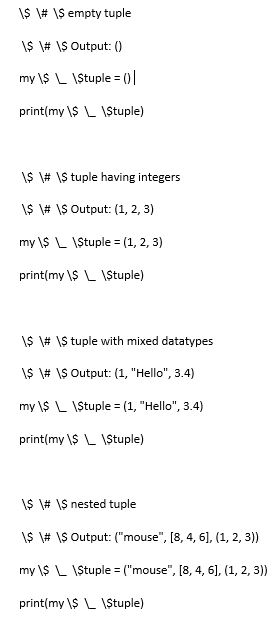
\includegraphics[width=0.1\textwidth]{figures/3afs1.JPG}}
			\caption{}
			\label{3afs1}
			\end{figure}
   
\begin{figure}[ht]
			\centerline{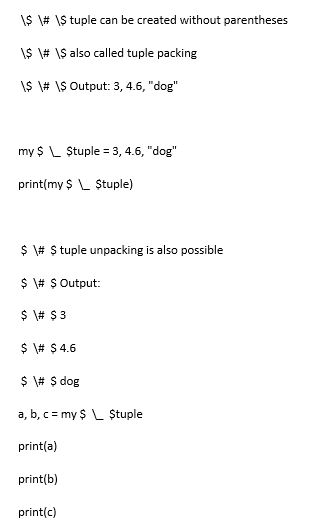
\includegraphics[width=0.1\textwidth]{figures/3afs2.JPG}}
			\caption{}
			\label{3afs2}
			\end{figure}
   

\section{Membuat tuple dengan satu elemen} 
Memiliki satu elemen dalam kurung saja tidak cukup. Kita membutuhkan koma trailing untuk menunjukkan bahwa sebenarnya ada tupel. 
\begin{verbatim}
 $  \#  $ only parentheses is not enough 
 $  \#  $ Output: <class 'str'> 
my $  \_  $tuple = ("hello") 
print(type(my $  \_  $tuple)) 

 $  \#  $ need a comma at the end 
 $  \#  $ Output: <class 'tuple'> 
my $  \_  $tuple~= ("hello",)   
print(type(my $  \_  $tuple)) 

 $  \#  $ parentheses is optional 
 $  \#  $ Output: <class 'tuple'> 
my $  \_  $tuple = "hello", 
print(type(my $  \_  $tuple)) 
\end{verbatim}
\section{Mengakses Elemen dalam Tuple} 
Ada berbagai cara untuk mengakses elemen tuple. 
\subsection{Pengindeksan}
Kita bisa menggunakan operator indeks [] untuk mengakses item di tupel dimana indeks dimulai dari 0. Jadi, tupel yang memiliki 6 elemen akan memiliki indeks dari 0 sampai 5. Mencoba mengakses elemen lain yang (6, 7, ...) akan menghasilkan IndexError. Indeks harus berupa bilangan bulat, jadi kita tidak bisa menggunakan float atau jenis lainnya. Ini akan menghasilkan TypeError. Demikian juga, tuple bersarang diakses menggunakan pengindeksan nested, seperti yang ditunjukkan pada contoh di bawah ini. 
\begin{verbatim}
my $  \_  $tuple = ('p','e','r','m','i','t') 

 $  \#  $ Output: 'p' 
print(my $  \_  $tuple[0]) \

 $  \#  $ Output: 't' 
print(my $  \_  $tuple[5]) 

 $  \#  $ index must be in range 
 $  \#  $ If you uncomment line 14, 
 $  \#  $ you will get an error. 
 $  \#  $ IndexError: list index out of range 

 $  \#  $print(my $  \_  $tuple[6]) 

 $  \#  $ index must be an integer 
 $  \#  $ If you uncomment line 21, 
 $  \#  $ you will get an error. 
 $  \#  $ TypeError: list indices must be integers, not float 

 $  \#  $my $  \_  $tuple[2.0] 

 $  \#  $ nested tuple 
n $  \_  $tuple = ("mouse", [8, 4, 6], (1, 2, 3)) 

 $  \#  $ nested index 
 $  \#  $ Output: 's' 
print(n $  \_  $tuple[0][3]) 

 $  \#  $ nested index 
 $  \#  $ Output: 4 
print(n $  \_  $tuple[1][1]) 
\end{verbatim}
\subsection{Slicing} 
Kita bisa mengakses berbagai item dalam tupel dengan menggunakan operator pengiris - titik dua ":". 
\begin{verbatim}
my $  \_  $tuple = ('p','r','o','g','r','a','m','i','z') 

 $  \#  $ elements 2nd to 4th 
 $  \#  $ Output: ('r', 'o', 'g') 
print(my $  \_  $tuple[1:4]) 

 $  \#  $ elements beginning to 2nd 
 $  \#  $ Output: ('p', 'r') 
print(my $  \_  $tuple[:-7]) 

 $  \#  $ elements 8th to end 
 $  \#  $ Output: ('i', 'z') 
print(my $  \_  $tuple[7:]) 

 $  \#  $ elements beginning to end 
 $  \#  $ Output: ('p', 'r', 'o', 'g', 'r', 'a', 'm', 'i', 'z') 
print(my $  \_  $tuple[:]) 
\end{verbatim}
\section{Mengubah Tuple} 
Tidak seperti daftar, tupel tidak dapat diubah. Ini berarti elemen tupel tidak dapat diubah begitu telah ditetapkan. Tapi, jika elemen itu sendiri adalah datatype yang bisa berubah seperti daftar, item nested-nya bisa diubah. Kita juga bisa menugaskan tuple ke nilai yang berbeda \(reassignment\). 
\begin{verbatim}
my $  \_  $tuple = (4, 2, 3, [6, 5]) 

 $  \#  $ we cannot change an element 
 $  \#  $ If you uncomment line 8 
 $  \#  $ you will get an error: 
 $  \#  $ TypeError: 'tuple' object does not support item assignment 

 $  \#  $my $  \_  $tuple[1] = 9 

 $  \#  $ but item of mutable element can be changed 
 $  \#  $ Output: (4, 2, 3, [9, 5]) 
my $  \_  $tuple[3][0] = 9 
print(my $  \_  $tuple) 

 $  \#  $ tuples can be reassigned 
 $  \#  $ Output: ('p', 'r', 'o', 'g', 'r', 'a', 'm', 'i', 'z') 
my $  \_  $tuple = ('p','r','o','g','r','a','m','i','z') 
print(my $  \_  $tuple) 
\end{verbatim}
\section{Python Tuples} 
Tutorial Tuple Python menjelaskan tupel dan bagaimana menggunakannya dengan Python. Dengan Python, tupel hampir sama dengan daftar. Jadi, mengapa kita harus menggunakannya? Satu perbedaan utama antara tupel dan daftar adalah bahwa tupel tidak dapat diubah. Artinya, Anda tidak dapat menambahkan, mengubah, atau menghapus elemen dari tuple. Tupel mungkin tampak aneh pada awalnya, tapi ada alasan bagus mengapa mereka tidak bisa berubah. Sebagai pemrogram, kita mengacaukan sesekali. Kami mengubah variabel yang tidak ingin kami ubah, dan terkadang, kami hanya ingin hal-hal menjadi konstan sehingga kami tidak sengaja mengubahnya nanti. Namun, jika kita mengubah pikiran kita, kita juga bisa mengubah tupel menjadi daftar atau daftar menjadi tupel. Faktanya adalah kita perlu membuat usaha sadar untuk mengatakan Python, saya ingin mengubah tupel ini menjadi sebuah daftar sehingga saya bisa memodifikasinya. Cukup mengoceh, mari kita lihat sebuah tuple beraksi!
Otak Anda masih sakit dari pelajaran terakhir? Jangan khawatir, yang satu ini akan membutuhkan sedikit pemikiran. Kita akan kembali ke sesuatu yang sederhana - variabel - tapi sedikit lebih mendalam. Pikirkanlah - variabel menyimpan satu bit informasi. Mereka mungkin muntah-muntah (tidak di karpet ...) informasi itu kapan saja, dan sedikit informasi mereka dapat berubah sewaktu-waktu. Variabel sangat bagus dengan apa yang mereka lakukan - menyimpan informasi yang mungkin berubah seiring berjalannya waktu. 

Tapi bagaimana jika Anda perlu menyimpan daftar panjang informasi, yang tidak berubah dari waktu ke waktu? Katakanlah, misalnya, nama bulan dalam setahun. Atau mungkin daftar panjang informasi, itu memang berubah seiring berjalannya waktu? Katakanlah, misalnya, nama semua kucing Anda. Anda mungkin mendapatkan kucing baru, beberapa mungkin mati, beberapa mungkin menjadi makan malam Anda (kami harus menukar resep!). Bagaimana dengan buku telepon? Untuk itu Anda perlu melakukan sedikit referensi - Anda akan memiliki daftar nama, dan dilampirkan pada masing-masing nama tersebut, nomor teleponnya. Bagaimana Anda melakukannya?

Untuk ketiga masalah ini, Python menggunakan tiga solusi berbeda - daftar, tupel, dan kamus: 
\begin{enumerate}
\item Daftar adalah apa yang mereka tampaknya - daftar nilai. Masing-masing diberi nomor, mulai dari nol - yang pertama diberi nomor nol, yang kedua 1, yang ketiga 2, dll. Anda dapat menghapus nilai dari daftar, dan menambahkan nilai baru sampai akhir. Contoh: nama kucing Anda banyak. 
\item Tupel sama seperti daftar, tapi Anda tidak dapat mengubah nilainya. Nilai yang Anda berikan terlebih dahulu, adalah nilai yang Anda pakai untuk sisa program. Sekali lagi, setiap nilai diberi nomor mulai dari nol, untuk referensi mudah. Contoh: nama bulan dalam setahun. 
\item Kamus serupa dengan apa yang namanya namanya - kamus. Dalam kamus, Anda memiliki 'indeks' kata-kata, dan untuk masing-masing definisi. Dengan kata Python, kata itu disebut 'kunci', dan definisi sebuah 'nilai'. Nilai dalam kamus tidak diberi nomor - keduanya tidak sesuai urutan tertentu, kuncinya adalah hal yang sama. (Setiap tombol harus unik, meskipun!) Anda dapat menambahkan, menghapus, dan memodifikasi nilai-nilai di kamus. Contoh: buku telepon jadi ada yang lebih hidup dari pada nama kucing Anda. Anda perlu menghubungi saudara perempuan, ibu, anak laki-laki, pria buah, dan orang lain yang perlu tahu bahwa kucing favorit mereka sudah meninggal. Untuk itu Anda membutuhkan buku telepon. 
\end{enumerate}
Sekarang, daftar yang telah kami gunakan di atas tidak sesuai untuk buku telepon. Anda perlu mengetahui nomor berdasarkan nama seseorang - bukan sebaliknya, seperti yang kami lakukan pada kucing. Dalam contoh bulan dan kucing, kami memberi nomor komputer, dan itu memberi kami sebuah nama. Kali ini kami ingin memberi nama komputer, dan ini memberi kami nomor. Untuk ini kita butuh kamus.

Jadi bagaimana kita membuat kamus? Letakkan peralatan pengikat Anda, bukan itu yang maju. ingat, kamus memiliki kunci, dan nilai. Dalam buku telepon, Anda punya nama orang, lalu nomor mereka. Melihat kesamaan? Saat pertama kali membuat kamus, sangat mirip membuat tupel atau daftar. Tupel memiliki (dan) benda, daftar memiliki [dan] benda. Tebak apa! kamus memiliki \$  \{  \$dan \$  \}  \$ hal - kurung kurawal. Berikut adalah contoh di bawah ini, menampilkan kamus dengan empat nomor telepon di dalamnya: 

Selain List, Tuple juga merupakan tipe data urutan \(sequence data type\) yang secara fungsi sama dengan List. Namun Tuple berbeda sifatnya, yaitu Tuple bersifat immutable yang mana data di dalam Tuple tidak dapat kita ubah atau dihapuskan. Sebuah Tuple terdiri dari beberapa nilai yang dipisahkan oleh tanda koma (‘,’). Tidak seperti List, tipe data Tuple ditandai dengan tanda kurung \"()\".

Tupel berguna untuk mewakili bahasa lain yang sering disebut catatan \- beberapa informasi terkait yang dimiliki bersama, seperti catatan siswa Anda. Tidak ada deskripsi tentang apa yang masing-masing bidang ini berarti, tapi kita bisa menebaknya. Sebuah tupel memungkinkan kita \"mengumpulkan\" informasi yang terkait dan menggunakannya sebagai satu hal.
